\documentclass[11pt,a4paper]{report}

\setlength\textwidth{145mm}
\setlength\textheight{247mm}
\setlength\oddsidemargin{15mm}
\setlength\evensidemargin{15mm}
\setlength\topmargin{0mm}
\setlength\headsep{0mm}
\setlength\headheight{0mm}
\let\openright=\clearpage

\usepackage[czech]{babel}
\usepackage{lmodern}
\usepackage[T1]{fontenc}
\usepackage{textcomp}

\usepackage[utf8]{inputenc}

\usepackage{stddoc}


\renewcommand{\vec}{\boldsymbol}
\def\endl{\\[3mm]}
\newcommand*\colvec[3][]{
	\begin{pmatrix}
		\ifx \relax#1 \relax
		\else #1\\
		\fi
		#2 \\ #3
	\end{pmatrix}
}


\makeatletter
\def\thmheadbrackets#1#2#3{%
	\thmname{#1}\thmnumber{\@ifnotempty{#1}{ }\@upn{#2}}%
	\thmnote{{\;\;\the\thm@notefont[#3]}}}
\makeatother

\newtheoremstyle{theorem}		% name
{\topsep}						% Space above
{\topsep}						% Space below
{\normalfont}					% Body font
{}								% Indent amount
{\bfseries}						% Theorem head font
{.}								% Punctuation after theorem head
{.5em}							% Space after theorem head
{\thmheadbrackets{#1}{#2}{#3}}	% theorem head spec

\theoremstyle{theorem}
\newtheorem{theorem}{Věta}[section]
\newtheorem{claim}{Tvrzení}[section]
\newtheorem*{example}{Příklad}
% The additional parameter [section] restarts the theorem counter at every new section.
\newtheorem{corollary}{Důsledek}[theorem]
% An environment called corollary is created, the counter of this new environment will be reset every time a new theorem environment is used.
\newtheorem{lemma}[theorem]{Lemma}
% In this case, the even though a new environment called lemma is created, it will use the same counter as the theorem environment.
\newtheorem*{observation}{Pozorování}
\newtheorem*{recap}{Opakování}

\theoremstyle{remark}
\newtheorem*{remark}{Poznámka}
\newtheorem*{solution}{Řešení}
\newtheorem*{convention}{Konvence}
% The syntax of the command \newtheorem* is the same as the non-starred version, except for the counter parameters. In this example a new unnumbered environment called remark is created.

\theoremstyle{definition}
\newtheorem{definition}{Definice}[section]



\begin{document}
	
	\pagenumbering{arabic}
	
	\section*{Speciální teorie relativity}
		
		\paragraph{Disclaimer.} Obrázek není mojí tvorbou, je vypůjčen ze skript pro Fyziku 1 od docenta Bednaříka, za což mu děkuji.
		
		\noindent
		Vyjdeme z Einsteinových postulátů speciální relativity
		\begin{enumerate}
			\item \textit{Všechny inerciální soustavy jsou si rovnocenné} (ve smyslu, že ve všech mají fyzikální zákony stejný tvar).
			
			\item \textit{Rychlost světla ve vakuu je ve všech inerciálních soustavách stejná.}
		\end{enumerate}
		
		\subsection*{Odvození Lorentzovy transformace}
			
			Jak jsme si již říkali, Maxwellovy rovnice elektromagnetismu vzbudili kontroverzi v řadách mnoha fyziků. Tato teorie, jejíž nepochybitelnost byla mnohokrát testována a potvrzena, totiž nebyla v souladu se základním chápáním pohybu, což byl Galileiho princip relativity. Tento základní stavební kámen Newtonovy mechaniky totiž stojí na faktu, že prostor a čas jsou invariantní (tj. neměnné) parametry popisu reality a tedy i nezávislé na pozorovatelích a jejich rychlostech. To byl však problém s Maxwellovými rovnicemi, kde se zdála být Galileova transformace (tj. přechod z popisu jednoho pozorovatele na druhého) neaplikovatelná.
			
			Přestavme si tedy modelovou situaci, kdy máme dvě soustavy, přičemž jedna z nich je v klidu (nečárkovaná soustava) a druhá (čárkovaná) se vůči ní pohybuje rychlostí $\vec V$ (viz Obrázek 1). My se tedy omezíme na jednorozměrný pohyb, a to na pohyb ve směru osy $x$. Galileova transformace říká, že
			\begin{align*}
				x' &= x-Vt,
			\\
				y' &= y,
			\\
				z' &= z,
			\\
				t' &= t.
			\end{align*}
			\begin{figure}[h!]
				\label{obr1}
				\begin{center}
					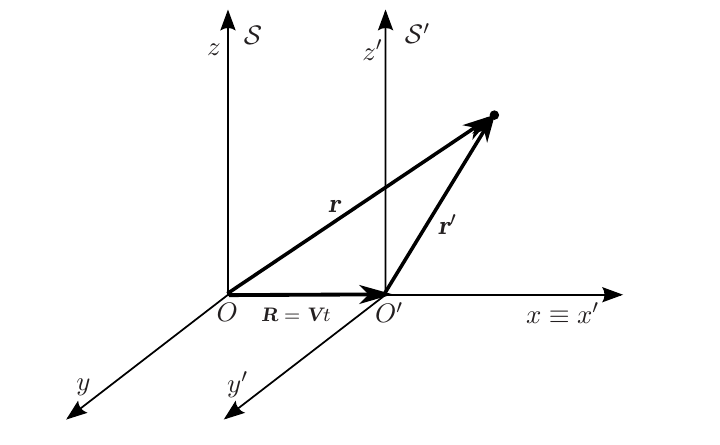
\includegraphics[width=0.75\linewidth]{img/1.png}
				\end{center}
				\caption{Ilustrační obrázek vzájemného pohybu soustav}
			\end{figure}
			
			My se však pokusíme vybudovat jinou transformaci, která bude postavena na Einsteinových postulátech. S využitím 1. postulátu speciální relativity (mezi soustavami bude možno přecházet pomocí lineárního vztahu, který však může být ovlivněn jakýmsi bezrozměrným koeficientem $\gamma$) napišme
			\begin{align}
				\label{eq:x-transform-nogamma}
				x' &= \gamma (x - Vt).
			\end{align}
			O souřadnicích $y$ a $z$ nic neříkáme, protože kvůli jejich nehybnosti platí triviálně $y'=y$ a $z'=z$. Zpětná transformace bude totožného rázu, kdy jediná změna bude v aktivní souřadnici $x = \gamma(x'-V't')$. Jelikož však víme, že tato rychlost $V'$ musí být opačná rychloti $V$,%
				\footnote{Stejně jako když stojíme u silnice a pozorujeme doprava jedoucí auto rychlostí $v$, řidíč auta dívající se stejným směrem vidí naopak vůči němu se doleva pohybující krajinu zase rychlostí $v$. Znamánko minus ve výrazu značí uvedenou změnu směru při přechodu do perspektivy druhého pozorovatele (řidiče).}
			můžeme psát $V' = -V$, tedy určitě platí
			\begin{align*}
				x &= \gamma (x'-V't') = \gamma (x'+Vt') = \gamma(\gamma (x - Vt) + Vt') = \gamma^2x - \gamma^2Vt + \gamma Vt'.
			\end{align*}
			Vyjádříme-li z krajních výrazů čárkovaný čas $t'$, dostáváme časovou transformaci
			\begin{align}
				\label{eq:time-transform-nogamma}
				t' &= \gamma t + \( \frac{1-\gamma^2}{\gamma V} \) x.
			\end{align}
			
		\subsubsection*{Lorentzův faktor $\gamma$}
			
			Předchozím postupem jsme získali mechanickou transformaci času a prostorových souřadnic, která je dozajista správná (např. dosazením za $\gamma = 1$ bychom získali i nám blízkou Galileovu transformaci). Zatím nám však není známo, jakých hodnot nabývá koeficient $\gamma$, tzv. \textit{Lorentzův faktor}. Pojďme se tedy pokusit o využití postulátů k tomu, abychom tento výraz určili. Druhý Einsteinův postulát (ten revoluční) nám říká, že rychlost světla ve vakuu je ve všech inerciálních soustavách stejná. Představme si tedy situaci podobnou té předchozí, akorát tentokrát bude trochu konkrétnější. Předpokládejme, že se naše soustavy nachází ve vakuu a v čase $t_o$, kdy se soustavy navzájem překrývají, vytryskne světelný paprsek pohybující se ve směru osy $x$ rychlostí světla $c = c'$. Einsteinův postulát nám říká, že tato rychlost musí být ve všech soustávách, tedy i těch našich, stejná. Můžeme tedy psát
			\begin{align}
				\label{eq:2nd-postulate}
				x &= c t,
			\\
				\label{eq:2nd-postulate'}
				x' &= c t'.
			\end{align}
			Dosadíme-li tedy do rovnice \eqref{eq:2nd-postulate'} nám již známé transformační vztahy \eqref{eq:x-transform-nogamma} a \eqref{eq:time-transform-nogamma}, dostáváme vyjádření ve tvaru
			\begin{align*}
				\gamma (x - Vt) &= c \[ \gamma t + \( \frac{1-\gamma^2}{\gamma V} \) x \],
			\\
				\gamma x - \gamma Vt &= c \gamma t + c \( \frac{1-\gamma^2}{\gamma V} \) x,
			\\
				x \[ \gamma - c \( \frac{1-\gamma^2}{\gamma V} \) \] &= \gamma (ct + Vt),
			\\
				x &= \frac{\gamma (ct + Vt)}{\gamma - c \frac{1-\gamma^2}{\gamma V}}.
			\end{align*}
			Toto se nezdá býti příliš příjemný výsledek, ale opak je pravdou. Vyjádříme-li z výsledného vztahu pro $x$ člen $ct$, dostaneme
			\begin{align*}
				x &= ct \frac{\gamma\(1 + \frac{V}{c}\)}{\gamma - c \frac{1-\gamma^2}{\gamma V}}.
			\end{align*}
			Vím, že to nevypadá o moc lépe, ale otevírá nám to možnost využít naplno síly druhého postulátu, který tvrdí, že pokud platí tato rovnost, tak právě ten nepříjemný koeficient za vytknutým členem $ct$ musí být roven 1, podle \eqref{eq:2nd-postulate}. Položíme-li ho tedy roven jedné, zbavíme se vlivu jak $x$, tak $t$ v rovnici a jedinou neznámou tak zůstává faktor $\gamma$, který se snažíme zjistit. Pomocí základních algebraických úprav se tak můžeme dostat až k výslednému vztahu ve tvaru
			\begin{align*}
				\frac{\gamma\(1 + \frac{V}{c}\)}{\gamma - c \frac{1-\gamma^2}{\gamma V}} &= 1,
			\\
				\gamma\(1 + \frac{V}{c}\) &= \gamma - c \frac{1-\gamma^2}{\gamma V},
			\\
				\gamma^2 Vc + \gamma^2 V^2 &= \gamma^2 Vc - c^2 + \gamma^2 c^2,
			\\
				\gamma^2(c^2-V^2) &= c^2,
			\\
				\gamma^2 &= \frac{c^2}{c^2 - V^2},
			\\
				\gamma^2 &= \frac{1}{1 - \frac{V^2}{c^2}},
			\\
				\Aboxed{\gamma &= \frac{1}{\sqrt{1 - \frac{V^2}{c^2}}}} \in \langle 1,\infty).
			\end{align*}
			Získali jsme tak finální podobu Lorentzova faktoru, který když dosadíme do transformačních vztahů \eqref{eq:x-transform-nogamma} a \eqref{eq:time-transform-nogamma}, dostáváme finální Lorentzovu transformaci, tedy
			\begin{align*}
				x' &= \gamma(x-Vt) = \frac{x-Vt}{\sqrt{1 - \frac{V^2}{c^2}}},
			\\
				t' &= \gamma t + \( \frac{1-\gamma^2}{\gamma V} \) x = \cdots = \frac{t-\frac{Vx}{c^2}}{\sqrt{1 - \frac{V^2}{c^2}}},
			\end{align*}
			přičemž zpětná transformace je analogického rázu ve tvaru
			\begin{align*}
				x &= \frac{x' + Vt'}{\sqrt{1 - \frac{V^2}{c^2}}},
			\\
				t &= \frac{t' + \frac{Vx'}{c^2}}{\sqrt{1 - \frac{V^2}{c^2}}}.
			\end{align*}
			
		\subsection*{Dilatace času a kontrakce délek}
			
			\paragraph*{Teoretický úvod.} Nyní uvažujme stejný systém jako na začátku, kdy do středu pohybující se čárkované soustavy položíme hodiny. Pro tyto hodiny platí, že $x'=0$, a čas uplynulý v čárkované soustavě $t'$ si označíme za tzv. \textit{vlastní čas} $T_0$ (vlastní čas proto, že je to čas uplynulý v soustavě, která je právě hodinám vlastní). Můžeme se však ptát na to, jaký časový interval za tuto dobu vnímá pozorovatel sedící v počátku soustavy v klidu (nečárkované). Jak jsme totiž ukázali, vnímání času není invariantem, nýbrž se může měnít v závislosti na soustavě, ve které se pozorovatel nachází, tedy na její rychlosti. Využitím předpokladu, že hodiny se nachází v počátku čárkované soustavy ($x'=0$), můžeme psát
			\begin{align*}
				x' &= \gamma(x-VT) = 0.
			\end{align*}
			Jelikož však známe tvar Lorentzova faktoru $\gamma$, víme že ten nulový nikdy být nemůže, musí být tedy nulová závorka, tedy platí $x=VT$. Pro vlastní čas $T_0$ uplynulý čárkované soustavě tedy můžeme psát
			\begin{align*}
				T_0 &= \gamma\(T - \frac{V^2 T}{c^2}\) = \gamma T\(1 - \frac{V^2}{c^2}\) = T \frac{\gamma}{\gamma^2} = \frac T \gamma,
			\end{align*}
			přičemž platí, že $\gamma > 1$, takže čas pozorovaný v libovolné soustavě jiné než čárkované je delší než čas vlastní. Dochází tedy k takzvané \textit{dilataci času} a odtud tedy známý vztah
			\begin{align*}
				\Aboxed{T_0 &= \frac T \gamma.}
			\end{align*}
			
			\begin{example}
				Při srážkách kosmického záření s atomy vrchní vrstvy atmosféry vznikají miony, což jsou nestabilní částice se střední dobou života $\tau_0 = 2,2 \cdot 10^{-6} \; \mathrm s$. Pozorování stratosferických balonů zjistila, že vznikají ve velkých výškách (více než 10 km) nad povrchem Země a odtud se pohybují směrem k zemskému povrchu rychlostí blízké rychlosti světla.
			\\
				Předpokládejme, že mion vznikl ve výšce 15 km nad zemským povrchem a řítí se k Zemi rychlostí $v = 0.999 \, c$. Mají šanci vědci pomocí pozemské stanice detekovat existenci tohoto mionu? Tedy, může tento mion doletět až na zemský povrch?
			\end{example}
			\begin{solution}
				Naším cílem bude spočítat celkovou možnou dráhu, kterou je mion schopen během svého života urazit. Z výše odvozeného vztahu pro dilataci času můžeme vidět, jak se transformuje časový interval pro pozemského pozorovatele, a to ve tvaru
				\begin{align*}
					\tau &= \tau_0 \gamma = \frac{\tau_0}{\sqrt{1 - \frac{V^2}{c^2}}}.
				\end{align*}
				Celková dráh, kterou je tedy schopen mion uletět před neodvratným rozpadem, je
				\begin{align*}
					l &= \frac{v\tau_0}{\sqrt{1 - \frac{V^2}{c^2}}} = \cdots = 32995 \ \mathrm m \approx 33 \ \mathrm{km},
				\end{align*}
				což vidíme, že je více než dvojnásobek potřebné dráhy pro to, abychom ho byli schopni na zemském povrchu detekovat. Finální odpovědí je tedy ano, je možné mion měřit na pozemské stanici, a to pouze díky speciální teorii relativity.
			\end{solution}
			
			Z nadpisu sekce je vidět, že souvisejícím jevem je také takzvaná \textit{kontrakce délek}. Ta má však odvození obdobné, takže pouze uvedeme vztah pro uvedenou kontrakci, tedy
			\begin{align*}
				\Aboxed{L_0 = \gamma L,}
			\end{align*}
			ze kterého je vidět, že tentokrát se symetricky naopak jedná o situaci, kdy \textit{vlastní délka} $L_0$ předmětu ve směru pohybu je vždy nejdelší a při vnímání tohoto rozměru z libovolné jiné soustavy dochází ke zkracování, tedy ke kontrakci.
		
\end{document}